% =============================================================================
% Chapter: Bayesian Networks
% =============================================================================

\chapter{Bayesian Networks}

\section{Εισαγωγή}

\keyword{Bayesian Networks} (BNs) είναι γραφικά μοντέλα που αναπαριστούν πιθανοτικές σχέσεις μεταξύ μεταβλητών. Χρησιμοποιούνται για uncertainty modeling και probabilistic inference.

\begin{definitionbox}[Bayesian Network]
\begin{itemize}
    \item \textbf{Directed Acyclic Graph (DAG)}: Κόμβοι = μεταβλητές, ακμές = εξαρτήσεις
    \item \textbf{Conditional Probability Tables (CPTs)}: Ορίζουν $P(X | \text{Parents}(X))$
    \item \textbf{Compact representation}: Εκμεταλλεύονται conditional independencies
\end{itemize}
\end{definitionbox}

% =============================================================================
\section{Bayes' Theorem}

\begin{formulabox}[Bayes' Theorem - ΑΠΟΜΝΗΜΟΝΕΥΣΕ!]
\begin{equation}
P(A|B) = \frac{P(B|A) \times P(A)}{P(B)}
\end{equation}

\begin{itemize}
    \item $P(A|B)$: \textbf{Posterior} (τι ξέρουμε μετά το evidence)
    \item $P(B|A)$: \textbf{Likelihood} (πόσο πιθανό το evidence δεδομένου A)
    \item $P(A)$: \textbf{Prior} (αρχική πεποίθηση)
    \item $P(B)$: \textbf{Marginal likelihood} (normalizer)
\end{itemize}

\textbf{Total Probability}:
\begin{equation}
P(B) = P(B|A) \times P(A) + P(B|\neg A) \times P(\neg A)
\end{equation}
\end{formulabox}

\begin{examplebox}[Medical Diagnosis]
\textbf{Δεδομένα}:
\begin{itemize}
    \item Disease: $P(D) = 0.01$ (1\% πληθυσμού)
    \item Test positive given disease: $P(+|D) = 0.95$
    \item Test positive given no disease: $P(+|\neg D) = 0.10$
\end{itemize}

\textbf{Ερώτηση}: Αν το test είναι positive, τι πιθανότητα έχω τη νόσο;

\begin{align*}
P(D|+) &= \frac{P(+|D) \times P(D)}{P(+)} \\
P(+) &= P(+|D) \times P(D) + P(+|\neg D) \times P(\neg D) \\
&= 0.95 \times 0.01 + 0.10 \times 0.99 = 0.0095 + 0.099 = 0.1085 \\
P(D|+) &= \frac{0.0095}{0.1085} = \boxed{0.0876 \approx 8.76\%}
\end{align*}

Μόνο $\sim$9\% παρά το 95\% accuracy του test! (λόγω χαμηλού prior - rare disease)
\end{examplebox}

% =============================================================================
\section{Bayesian Network Structure}

\begin{center}
\begin{tikzpicture}[
    node distance=1.5cm,
    bn node/.style={
        circle,
        draw=primary,
        fill=box-blue,
        minimum size=1.5cm,
        font=\small
    }
]
    % Nodes
    \node[bn node] (B) {Burglary};
    \node[bn node, right=2cm of B] (E) {Earthquake};
    \node[bn node, below=1.5cm of $(B)!0.5!(E)$] (A) {Alarm};
    \node[bn node, below left=1.5cm of A] (J) {JohnCalls};
    \node[bn node, below right=1.5cm of A] (M) {MaryCalls};

    % Edges
    \draw[->, >=Stealth, thick] (B) -- (A);
    \draw[->, >=Stealth, thick] (E) -- (A);
    \draw[->, >=Stealth, thick] (A) -- (J);
    \draw[->, >=Stealth, thick] (A) -- (M);

    % Legend
    \node[anchor=north west, align=left, font=\small] at (6,-1) {
        \textbf{Ερμηνεία}:\\
        Alarm ενεργοποιείται από\\
        Burglary ή Earthquake\\[0.5em]
        John/Mary καλούν όταν\\
        ακούν Alarm
    };
\end{tikzpicture}
\end{center}

% =============================================================================
\section{Conditional Probability Tables (CPTs)}

\begin{center}
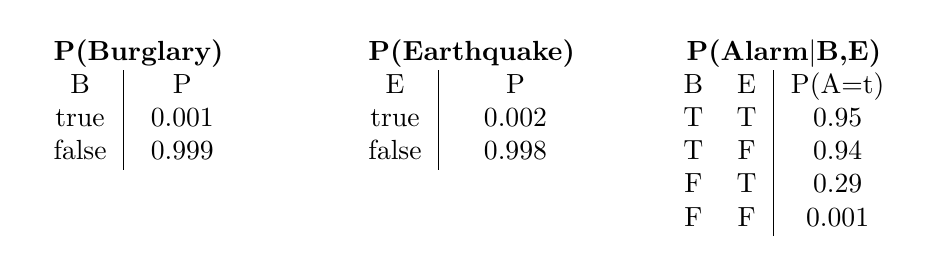
\begin{tikzpicture}
    % P(Burglary) table
    \node[anchor=north west] at (0,0) {
        \begin{tabular}{c|c}
            \multicolumn{2}{c}{\textbf{P(Burglary)}} \\
            \toprule
            B & P \\
            \midrule
            true & 0.001 \\
            false & 0.999 \\
            \bottomrule
        \end{tabular}
    };

    % P(Earthquake) table
    \node[anchor=north west] at (4,0) {
        \begin{tabular}{c|c}
            \multicolumn{2}{c}{\textbf{P(Earthquake)}} \\
            \toprule
            E & P \\
            \midrule
            true & 0.002 \\
            false & 0.998 \\
            \bottomrule
        \end{tabular}
    };

    % P(Alarm | B, E) table
    \node[anchor=north west] at (8,0) {
        \begin{tabular}{cc|c}
            \multicolumn{3}{c}{\textbf{P(Alarm$|$B,E)}} \\
            \toprule
            B & E & P(A=t) \\
            \midrule
            T & T & 0.95 \\
            T & F & 0.94 \\
            F & T & 0.29 \\
            F & F & 0.001 \\
            \bottomrule
        \end{tabular}
    };
\end{tikzpicture}
\end{center}

\begin{infobox}[CPT Size]
Node X με binary parents $P_1, P_2, \ldots, P_k$:

\textbf{CPT rows} = $2^k$

Παράδειγμα: Alarm με 2 binary parents $\Rightarrow$ 4 rows
\end{infobox}

% =============================================================================
\section{Joint Probability (Chain Rule)}

\begin{formulabox}[Chain Rule για Bayesian Networks]
\begin{equation}
P(X_1, X_2, \ldots, X_n) = \prod_{i=1}^{n} P(X_i | \text{Parents}(X_i))
\end{equation}

\textbf{Για το Alarm network}:
\[
P(B,E,A,J,M) = P(B) \times P(E) \times P(A|B,E) \times P(J|A) \times P(M|A)
\]
\end{formulabox}

\begin{examplebox}[Joint Probability Calculation]
$P(b, \neg e, a, j, m)$ = ?

\begin{align*}
&= P(b) \times P(\neg e) \times P(a|b,\neg e) \times P(j|a) \times P(m|a) \\
&= 0.001 \times 0.998 \times 0.94 \times 0.90 \times 0.70 \\
&= \boxed{0.000591}
\end{align*}
\end{examplebox}

% =============================================================================
\section{D-Separation (Conditional Independence)}

\begin{center}
\begin{tikzpicture}
    % Serial
    \node[draw=secondary, fill=secondary!20, rounded corners=10pt, minimum width=4cm, minimum height=3cm] (serial) at (0,0) {};
    \node[anchor=north, font=\bfseries\color{secondary}] at (serial.north) {Serial (Chain)};
    \node[circle, draw=primary, fill=box-blue, minimum size=0.8cm] (sa) at (-1,0) {A};
    \node[circle, draw=primary, fill=box-blue, minimum size=0.8cm] (sb) at (0,0) {B};
    \node[circle, draw=primary, fill=box-blue, minimum size=0.8cm] (sc) at (1,0) {C};
    \draw[->, >=Stealth, thick] (sa) -- (sb);
    \draw[->, >=Stealth, thick] (sb) -- (sc);
    \node[font=\small, anchor=north] at (serial.south) {$A \perp C | B$};

    % Diverging
    \node[draw=info, fill=info!20, rounded corners=10pt, minimum width=4cm, minimum height=3cm] (div) at (5.5,0) {};
    \node[anchor=north, font=\bfseries\color{info}] at (div.north) {Diverging};
    \node[circle, draw=primary, fill=box-blue, minimum size=0.8cm] (da) at (4.5,0) {A};
    \node[circle, draw=primary, fill=box-blue, minimum size=0.8cm] (db) at (5.5,0.8) {B};
    \node[circle, draw=primary, fill=box-blue, minimum size=0.8cm] (dc) at (6.5,0) {C};
    \draw[<-, >=Stealth, thick] (da) -- (db);
    \draw[->, >=Stealth, thick] (db) -- (dc);
    \node[font=\small, anchor=north] at (div.south) {$A \perp C | B$};

    % Converging (V-structure)
    \node[draw=accent, fill=accent!20, rounded corners=10pt, minimum width=4cm, minimum height=3cm] (conv) at (11,0) {};
    \node[anchor=north, font=\bfseries\color{accent}] at (conv.north) {Converging (V)};
    \node[circle, draw=primary, fill=box-blue, minimum size=0.8cm] (ca) at (10,0.3) {A};
    \node[circle, draw=primary, fill=box-blue, minimum size=0.8cm] (cb) at (11,-0.5) {B};
    \node[circle, draw=primary, fill=box-blue, minimum size=0.8cm] (cc) at (12,0.3) {C};
    \draw[->, >=Stealth, thick] (ca) -- (cb);
    \draw[->, >=Stealth, thick] (cc) -- (cb);
    \node[font=\small, anchor=north, align=center] at (conv.south) {$A \perp C$ (χωρίς evidence)\\$A \not\perp C | B$};
\end{tikzpicture}
\end{center}

\begin{warningbox}[D-Separation Rules - ΑΠΟΜΝΗΜΟΝΕΥΣΕ!]
\begin{center}
\begin{tabular}{lll}
\toprule
\textbf{Structure} & \textbf{B unknown} & \textbf{B known} \\
\midrule
Serial: $A \to B \to C$ & Open & \textcolor{success}{Blocked} \\
Diverging: $A \leftarrow B \to C$ & Open & \textcolor{success}{Blocked} \\
Converging: $A \to B \leftarrow C$ & \textcolor{success}{Blocked} & Open (explaining away!) \\
\bottomrule
\end{tabular}
\end{center}
\end{warningbox}

\begin{infobox}[Explaining Away]
Σε V-structure $A \to C \leftarrow B$, αν γνωρίζουμε $C=\text{true}$:
\begin{itemize}
    \item Αρχικά: A, B ανεξάρτητα
    \item Μετά: αν μάθουμε $A=\text{true}$ (μία αιτία του C), η $P(B=\text{true})$ \textbf{μειώνεται}
\end{itemize}
Το A "εξηγεί" το C, οπότε χρειαζόμαστε λιγότερο το B.
\end{infobox}

% =============================================================================
\section{Naive Bayes Classifier}

\begin{center}
\begin{tikzpicture}[
    node distance=1.2cm,
    bn node/.style={
        circle,
        draw=primary,
        fill=box-blue,
        minimum size=1.2cm,
        font=\small
    }
]
    % Class node
    \node[bn node, fill=secondary!30] (C) {Class};

    % Feature nodes
    \node[bn node, below left=1.5cm and 1cm of C] (X1) {$X_1$};
    \node[bn node, below=1.5cm of C] (X2) {$X_2$};
    \node[bn node, below right=1.5cm and 1cm of C] (X3) {$X_3$};

    % Edges
    \draw[->, >=Stealth, thick] (C) -- (X1);
    \draw[->, >=Stealth, thick] (C) -- (X2);
    \draw[->, >=Stealth, thick] (C) -- (X3);

    % Assumption
    \node[anchor=west, align=left] at (4,0) {
        \textbf{Naive Assumption}:\\
        Features $X_1, X_2, \ldots$ are\\
        \textit{conditionally independent}\\
        given Class
    };
\end{tikzpicture}
\end{center}

\begin{formulabox}[Naive Bayes Classification]
\begin{equation}
P(C|X_1, \ldots, X_n) \propto P(C) \times \prod_i P(X_i|C)
\end{equation}

\textbf{Prediction}:
\[
\hat{C} = \arg\max_C \left[ P(C) \times \prod_i P(X_i|C) \right]
\]
\end{formulabox}

\begin{examplebox}[Spam Classification]
\textbf{Training data}: 40 Spam, 60 Ham
\begin{itemize}
    \item P(Spam) = 0.4, P(Ham) = 0.6
    \item P("free"|Spam) = 0.75, P("free"|Ham) = 0.10
    \item P("money"|Spam) = 0.50, P("money"|Ham) = 0.05
\end{itemize}

\textbf{New email} contains "free" and "money":
\begin{align*}
P(\text{Spam}|\text{free,money}) &\propto 0.4 \times 0.75 \times 0.50 = 0.15 \\
P(\text{Ham}|\text{free,money}) &\propto 0.6 \times 0.10 \times 0.05 = 0.003 \\[0.5em]
P(\text{Spam}|\ldots) &= \frac{0.15}{0.15 + 0.003} = 0.98 \Rightarrow \boxed{\text{SPAM!}}
\end{align*}
\end{examplebox}

% =============================================================================
\section{Συχνά Λάθη}

\begin{warningbox}[Κοινά Λάθη στις Εξετάσεις]
\begin{enumerate}
    \item \textbf{Bayes' Rule}:
    \begin{itemize}
        \item[$\times$] $P(A|B) = P(B|A)$
        \item[\checkmark] $P(A|B) = P(B|A) \times P(A) / P(B)$
    \end{itemize}

    \item \textbf{Base Rate Neglect}:
    \begin{itemize}
        \item[$\times$] Test 95\% accurate $\Rightarrow$ $P(D|+) \approx 95\%$
        \item[\checkmark] Εξαρτάται ΠΟΛΥ από $P(D)$ (prior)!
    \end{itemize}

    \item \textbf{CPT Probabilities}:
    \begin{itemize}
        \item[$\times$] $P(A=t|B=t) + P(A=t|B=f) = 1$
        \item[\checkmark] $P(A=t|B=t) + P(A=f|B=t) = 1$ (sum over output!)
    \end{itemize}
\end{enumerate}
\end{warningbox}

% =============================================================================
\section{Σύνοψη - Key Points}

\begin{center}
\begin{tikzpicture}
    \node[draw=ntua-blue, fill=ntua-blue!10, rounded corners=5pt, minimum width=14cm, minimum height=9cm] (main) at (0,0) {};

    % Bayes' Theorem
    \node[anchor=north west, font=\bfseries\Large\color{ntua-blue}] at ([xshift=5pt, yshift=-5pt]main.north west) {Bayes' Theorem};
    \node[anchor=north west, align=left] at ([xshift=10pt, yshift=-35pt]main.north west) {
        $P(A|B) = \frac{P(B|A) \times P(A)}{P(B)}$\\[0.5em]
        $P(B) = P(B|A) \cdot P(A) + P(B|\neg A) \cdot P(\neg A)$
    };

    % Chain Rule
    \node[anchor=north west, font=\bfseries\color{secondary}] at ([xshift=8cm, yshift=-5pt]main.north west) {Chain Rule};
    \node[anchor=north west, align=left, font=\small] at ([xshift=8cm, yshift=-25pt]main.north west) {
        $P(X_1, \ldots, X_n) = \prod_i P(X_i | \text{Pa}(X_i))$
    };

    % D-Separation box
    \node[draw=secondary, fill=box-blue, rounded corners=5pt, minimum width=12cm, minimum height=2.5cm]
        at (0,-1) {};
    \node[anchor=north, font=\bfseries\color{secondary}] at (0,0.2) {D-Separation};
    \node[align=center, font=\small] at (0,-1.2) {
        Serial: $A \to B \to C$ $\Rightarrow$ $A \perp C | B$ (blocked when B known)\\
        Diverging: $A \leftarrow B \to C$ $\Rightarrow$ $A \perp C | B$ (blocked when B known)\\
        Converging: $A \to B \leftarrow C$ $\Rightarrow$ $A \perp C$ (blocked when B \textit{unknown}!)
    };

    % Naive Bayes box
    \node[draw=success, fill=box-green, rounded corners=5pt, minimum width=6cm, minimum height=2cm]
        at (-3,-3.5) {};
    \node[align=center, font=\small] at (-3,-3.5) {
        \textbf{Naive Bayes}\\
        $P(C|X) \propto P(C) \times \prod_i P(X_i|C)$
    };

    % CPT Size box
    \node[draw=info, fill=info!20, rounded corners=5pt, minimum width=5cm, minimum height=2cm]
        at (4,-3.5) {};
    \node[align=center, font=\small] at (4,-3.5) {
        \textbf{CPT Size}\\
        $k$ binary parents $\Rightarrow 2^k$ rows
    };
\end{tikzpicture}
\end{center}
